\section{Resultados e Deduções}\label{result}

Para a verificação dos resultados, são necessárias, em suma, duas preocupações principais. A primeira é de interpretação da teoria quantica da luz, e perceber seu comportamento de onda. A segunda é a verificação prática do comprimento de onda do laser utilizado, por meio das medidas e dados coletados. Se o comprimento de onda corresponder com a cor de laser usado no experimento, o experimento passa a ter um resultado positivo.

\subsection{Fenda Simples}\label{fenda_simples}

Na fenda simples verificamos, sem partir para medições, que a luz do laser difrata ao passar pela fenda que tem expessura menor que seu diâmetro. Isso já indica de cara um comportamento de onda para a luz. Também verificamos uma padrão em que se repetem pontos claros e escuros, totalmente simétricos, e com ponto mais claro no centro, passando a perder intensidade ao chegar para as extremidades. A propagação das ondas para a área de sombra pode ser explicada por considerar pequenos elementos da frente de onda na fenda e tratá-los como fontes pontuais. Dessa forma, os raios dessas fontes pontuais passam a sofrer interferencia uns dos outros.

Uma das características da difracção da fenda simples é que uma fenda estreita irá dar um padrão de difracção mais amplo, o que parece um pouco contra-intuitivo. Uma forma de visualização é de considerar que os raios da extremidade devem atingir meio comprimento de onda ($\frac{\lambda}{2}$) de diferença no comprimento da tragetória da luz, e, se a fenda é mais estreita, vai demorar um ângulo maior para os os raios alcançarem essa diferença.

Para chegar à equação que ajudará a achar o comprimento de onda do laser utilizado em função das medidas encontradas ao fazer o experimento, e então comparar esse comprimento de onda ao intervalo que faz sentido pra cor de laser que foi usado, temos que primeiramente fazer algumas aproximações.

\begin{figure}[H]
\begin{center}
\begin{tikzpicture}[decoration=penciline, decorate,scale=1]
	\draw[thick] (0,0) -- (0,0.9) ; % barra de baixo
	\draw[thick] (0,1.1) -- (0,2) ; % barra de cima
	% ondas primarias
	\foreach \A in {0,0.1,0.2,0.3,0.4,0.5} {
		\draw[thick] (-0.8 + \A,0.5) -- (-0.8 + \A,1.5) ;
	}
\end{tikzpicture}
\end{center}
\caption{Frentes planas e paralelas}
\label{frentes}
\end{figure}

Prieiro é necessário considerar que a luz do laser está vindo de uma fonte infinitamente distante, para considerar frentes de onda planas e paralelas entre si. Isso garante que os elementos de amplitude estejam em fase.


\begin{figure}[H]
\begin{center}
\begin{tikzpicture}[decoration=penciline, decorate,scale=1]
	\draw[thick] (0,0) -- (0,2.4) ; % barra de baixo
	\draw[thick] (0,2.6) -- (0,5) ; % barra de cima
	\draw[thick] (5,0) -- (5,5) ; 	% parede
	%padrão deluz na parede
	\draw[thick,color=red,fill=red] (5.2,2.5) ellipse (0.05 and 0.4);
	\draw[thick,color=red,fill=red] (5.2,3.3) ellipse (0.05 and 0.3);
	\draw[thick,color=red,fill=red] (5.2,1.7) ellipse (0.05 and 0.3);
	\draw[thick,color=red,fill=red] (5.2,4.05) ellipse (0.05 and 0.2);
	\draw[thick,color=red,fill=red] (5.2,0.95) ellipse (0.05 and 0.2);
	%diametro da fresta
	\draw[thick] (-0.2,2.4) -- (-0.2,2.6) ; 
	\draw[thick] (-0.3,2.6) -- (-0.1,2.6) ;
	\draw[thick] (-0.3,2.4) -- (-0.1,2.4) ;
	\node[black,scale=1] at (-0.45,2.44) {$a$};
	%distancia entre fenda e parede
	\draw[dashed]  (0.0,-0.3) -- (5.0,-0.3) ;
	\draw[thick]  (0.0,-0.2) -- (0.0,-0.4) ;	
	\draw[thick]  (5.0,-0.2) -- (5.0,-0.4) ;	
	\node[black,scale=1] at (2.5,-0.6) {$D$};
	%distancia y
	\draw[dashed]  (4.8,2.5) -- (4.8,3.75) ;
	\draw[thick]  (4.7,2.5) -- (4.9,2.5) ;
	\draw[thick]  (4.7,3.75) -- (4.9,3.75) ;
	\node[black,scale=1] at (4.58,3.125) {$y$};
	%mostra do angulo
	\draw[dashed]  (0,2.5) -- (5,3.75) ;
	\draw[dashed]  (0,2.5) -- (2.5,2.5) ;
	\node[black,scale=1] at (1.3,2.66) {$\theta$};
\end{tikzpicture}
\end{center}
\caption{Difração em fenda simples}
\label{diff_simples}
\end{figure}



Em seguida considerando que $\tan \theta =\frac{y}{D}$, podemos considerar que $D>>a$ (em algumas das nossas medições $D$ teve quase 9 metros, sendo que em uma delas teve quase 30, e a fenda sempre teve poucos milimetros), e assim podemos fazer aproximações $\tan\theta \approx \sin \theta \approx \theta \approx \frac{y}{D}$. Considerando então que $a \sin \theta =m\lambda$, então $a\frac{y}{D} =m\lambda$ e por fim:

\begin{equation}\label{eq_simples}
	\lambda \approx \frac{ya}{mD}
\end{equation}

Sendo $a$ o diâmetro da fenda, $m$ a quantidade de pontos escuros a partir do centro, $D$ a distância da fenda até o ponto de leitura, e $y$ a distância do centro luminoso até ultimo ponto de leitura.

\end{multicols}

\vspace{2cm}
\begin{center}
\begin{tikzpicture}[scale=1.5]
%	\draw[very thin,color=gray] (-0.1,-0.1) grid (9*0.7+0.9,8*0.7+0.9);

	\draw[->] (-0.2,0) -- (9*0.7+1,0) node[below left] {$x$};
	\draw[->] (0,-0.2) -- (0,8*0.7+1) node[right] {$f(x)$};

	\tikz \draw plot[smooth] file {./simples.table};
\end{tikzpicture}
\vspace{1.5cm}
\\\hypertarget{diagrama}{Dados capturados - Fenda Simples}
\end{center}

\begin{multicols}{2}    % 2 columns

Na figura acima vemos o padrão luminoso que capturamos para o laser verde. É um gráfico intensidade vs. tempo. Foram capturados 6 pontos escuros para cada lado, esses pontos simétricos ao centro. A distância do laser para a fenda (que não entra para os cálculos) foi de $17,16 mm$. A distancia $D$ da fenda até a parede (ponto de leitura) foi de $8,94m \pm 1cm$, e o percurso todo de leitura $2y$ foi de $115.23cm \pm 1cm$. Nossa fenda simples possui abertura de $0,05mm \pm 0,04mm$.

Basta agora aplicarmos a equação aproximada para verificar se o comprimento de onda $\lambda$ corresponde a um intervalo coerente com a cor verde.

\begin{align*}\label{calc_simples}
\lambda & \approx \frac{ya}{mD}\\
&\approx \frac{0,576\cdot 0,00005}{6 \cdot 8,94}\\
&\approx 536.9127517\cdot 10^{-9}\\
&\approx 536.9127517\cdot 10^{-9} \pm 446.1254589\cdot 10^{-9}
\end{align*}



É notável o erro imenso que foi carregado para o resultado final. Isso se deve aos instrumentos de medição não profissionais utilizados. Entretanto, os valores sem a consideração do erro batem com o esperado, tendo comprimento de onda $\lambda$ dentro do intervalo da cor verde $\lambda 500-565 nm$

\begin{equation}\label{sinal}
	I(\beta)=I_0 \frac{sin^2\beta}{\beta^2}
\end{equation}
Sendo $I_0$ o valor de intensidade máxima da luz observado no intervalo $\beta$, obtendo assim valores mínimos para $\beta=\pm n \pi$ e valores máximos relativos nas raízes de $\beta=tg(\beta)$.\cite{ondas}

\subsection{Fenda Dupla}\label{fenda_dupla}
\begin{equation}
	\lambda \approx \frac{yd}{mD}
\end{equation}
Sendo $d$ o diâmetro do conjunto fenda-fenda, $m$ a quantidade de pontos escuros a partir do centro, $D$ a distância da fenda até o ponto de leitura, e $y$ a distância do centro luminoso até ultimo ponto de leitura.
%soh esqueleto pra continuar dps